\section{Systèmes d'équations différentielles}

\subsection{Systèmes d'équations différentielles linéaires}

\compileSOL{\SOLUb}{\ref{18Q1}}{
\subQ{a} Nous avons les valeurs propres et vecteurs propres suivants.
\begin{center}
\begin{tabular}{l|l}
valeur propre & un vecteur propre \\
\hline
\rule{0em}{1.4em} $\lambda_1 = -5$ & $\displaystyle \VEC{v}_1 =
\begin{pmatrix} -2 & 1 \end{pmatrix}^\top$ \\[0.5em]
$\lambda_2 = 7$ & $\displaystyle \VEC{v}_2 =
\begin{pmatrix} 2 & 1 \end{pmatrix}^\top$
\end{tabular}
\end{center}
La solution générale est donc de la forme
\[
\VEC{x} = \alpha e^{\lambda_1 t}\VEC{v}_1 
+ \beta e^{\lambda_2 t}\VEC{v}_2
=  \alpha e^{-5 t} \begin{pmatrix} -2 \\ 1 \end{pmatrix}
+ \beta e^{7 t}\begin{pmatrix} 2 \\ 1 \end{pmatrix}
= \begin{pmatrix}
-2 \alpha e^{-5 t} + 2 \beta e^{7t} \\
\alpha e^{-5 t} + \beta e^{7t}
\end{pmatrix} \ .
\]
Pour satisfaire la condition initiale
$\displaystyle \begin{pmatrix} 0 & 1 \end{pmatrix}^\top$ à $t=0$, il
faut choisir $\alpha$ et $\beta$ de telle sorte que
\[
\begin{pmatrix} 0 \\ 1 \end{pmatrix} = \begin{pmatrix}
-2 \alpha + 2 \beta \\ \alpha + \beta \end{pmatrix} \ .
\]
C'est-à-dire, $-2\alpha + 2\beta = 0$ et $\alpha + \beta =1$.  La première
équation donne $\beta = \alpha$.  Si nous substituons $\beta=\alpha$ dans
l'équation $\alpha + \beta =1$, nous obtenons
$\displaystyle \alpha = \beta = 1/2$.  La solution qui satisfait la
condition initiale est
\[
\VEC{x} = \begin{pmatrix}
- e^{-5 t} + e^{7t} \\
\displaystyle \frac{1}{2} e^{-5 t} + \frac{1}{2} e^{7t}
\end{pmatrix} \ .
\]
Puisque $\lambda_1 < 0 < \lambda_2$, les deux valeurs propres sont de
signes opposés, nous obtenons le portrait de phases suivant.
\PDFgraph{18_syst_equ_diff/portrait1}
Pour nous aider à tracer le portrait de phases, nous avons aussi
inclus les nullclines avec la direction dans chacune des régions
du plan découpées par les nullclines.

\subQ{c} Il y a une seule valeur propre et tous les vecteurs
propres associés à cette valeur propre sont des multiples du vecteur
que nous avons choisi comme vecteur propre dans notre tableau.
\begin{center}
\begin{tabular}{l|l}
valeur propre & un vecteur propre \\
\hline
\rule{0em}{1.4em}
$\lambda = -1$ &
$\displaystyle \VEC{v} =\begin{pmatrix} 1 & -1 \end{pmatrix}^\top$
\end{tabular}
\end{center}
Il faut donc trouver un vecteur $\VEC{u}$ tel que $(A+\Id)\VEC{u} = \VEC{v}$.
Si nous posons
$\displaystyle \VEC{u} = \begin{pmatrix} a & b \end{pmatrix}^\top$, il
faut résoudre le système d'équations linéaires
\[
\begin{pmatrix} 1 & 1 \\ -1 & -1 \end{pmatrix}
\begin{pmatrix} a \\ b \end{pmatrix} =
\begin{pmatrix} 1 \\ -1 \end{pmatrix} \ .
\]
La matrice augmentée est
\[
\left(
\begin{array}{cc|c}
1 & 1 & 1 \\
-1 & -1 & -1
\end{array}\right) \ .
\]
$R_2+R_1 \rightarrow R_1$ donne
\[
\left(
\begin{array}{cc|c}
1 & 1 & 1 \\
0 & 0 & 0
\end{array}\right) \ .
\]
Ainsi $a + b = 1$.  Si $a=1$, alors $b=0$.  Nous obtenons le vecteur
$\displaystyle \VEC{u} = \begin{pmatrix} 1 & 0 \end{pmatrix}^\top$.

La solution générale est donc de la forme
\begin{align*}
\VEC{x} &= \alpha e^{\lambda t}\VEC{v} 
+ \beta e^{\lambda t} \left(\VEC{u} + t \VEC{v}\right)
=  \alpha e^{-t} \begin{pmatrix} 1 \\ -1 \end{pmatrix}
+ \beta e^{-t}\left( \begin{pmatrix} 1 \\ 0 \end{pmatrix}
+t \begin{pmatrix} 1 \\ -1 \end{pmatrix} \right) \\
&= \begin{pmatrix}
\alpha e^{-t} + \beta e^{-t}(1+t) \\
- \alpha e^{-t} - \beta e^{-t}t
\end{pmatrix} \ .
\end{align*}
Pour satisfaire la condition initiale
$\displaystyle \begin{pmatrix} 0 \\ 1 \end{pmatrix}$ à $t=0$, il faut
choisir $\alpha$ et $\beta$ de telle sorte que
\[
\begin{pmatrix} 0 \\ 1 \end{pmatrix} = \begin{pmatrix}
\alpha + \beta \\ -\alpha \end{pmatrix} \ .
\]
Nous trouvons $\alpha = -1$ et $\beta = 1$.  La solution qui
satisfait la condition initiale est
\[
\VEC{x} = \begin{pmatrix}
-e^{-t} + e^{-t}(1+t) \\
e^{-t} - e^{-t}t
\end{pmatrix}  \ .
\]

Puisque la seule valeur propre, $\lambda_1$, est négative, nous obtenons
le portrait de phases suivant.
\PDFgraph{18_syst_equ_diff/portrait2}
Pour nous aider à tracer le portrait de phases, nous avons aussi
inclus les nullclines avec la direction dans chacune des régions
du plan découpées par les nullclines.
}

\subsection{Analyse global}

\compileSOL{\SOLUb}{\ref{18Q2}}{
\subQ{a} Nous avons un système d'équations différentielles de la forme
\[
  \begin{pmatrix}
   x ' \\ y'
  \end{pmatrix} = \VEC{f}(x,y)
\]
avec $f_1(x,y) = 4x+y +25$ et $f_2(x,y) = 3x+2y+15$.

\subI{I} Le nullcline associé à $x$ est la droite
$f_1(x,y) = 4x + y + 25 = 0$ et le
nullcline associé à $y$ est la droite $f_2(x,y) = 3x + 2y + 15 = 0$.

\subI{II} Pour trouver le point d'équilibre de ce système d´équations
différentielles, il faut résoudre le système d'équations linéaires
\[
\begin{split}
f_1(x,y) = 4x+y + 25 &= 0 \\
f_2(x,y) = 3x+2y + 15 &=0
\end{split} \qquad \Leftrightarrow \qquad 
\begin{split}
4x+y &= -25 \\
3x+2y &= -15
\end{split}
\]
La matrice augmenté du système est
\[
\left(\begin{array}{cc|c}
4 & 1 & -25 \\ 3 & 2 & -15
\end{array}\right) \ .
\]
$R_1-R_2 \rightarrow R_1$ donne
\[
\left(\begin{array}{cc|c}
1 & -1 & -10 \\ 3 & 2 & -15
\end{array}\right) \ .
\]
$R_2-3R_1\rightarrow R_2$ donne
\[
\left(\begin{array}{cc|c}
1 & -1 & -10 \\ 0 & 5 & 15
\end{array}\right) \ .
\]
$(1/5)R_2 \rightarrow R_2$ donne
\[
\left(\begin{array}{cc|c}
1 & -1 & -10 \\ 0 & 1 & 3
\end{array}\right) \ .
\]
Finalement, $R_1+R_2 \rightarrow R_1$ donne
\[
\left(\begin{array}{cc|c}
1 & 0 & -7 \\ 0 & 1 & 3
\end{array}\right) \ .
\]
La solution est $x=-7$ et $y=3$.  Il y a un seul point d'équilibre qui est
$\VEC{p} = \begin{pmatrix} -7 \\ 3 \end{pmatrix}$.  C'est le point
d'intersection des deux nullclines.

\subI{III} La dérivée de $f$ est
\[
\diff \VEC{f}(x,y) =
\begin{pmatrix}
\displaystyle \pdydx{f_1}{x}(x,y) & \displaystyle \pdydx{f_1}{y}(x,y) \\[0.8em]
\displaystyle \pdydx{f_2}{x}(x,y) & \displaystyle \pdydx{f_2}{y}(x,y)
\end{pmatrix}
= \begin{pmatrix} 4 & 1 \\ 3 & 2 \end{pmatrix} \ .
\]
Si nous évaluons au point $\VEC{p}$, nous trouvons naturellement
\[
  \diff \VEC{f}(\VEC{p}) =
  \begin{pmatrix} 4 & 1 \\ 3 & 2 \end{pmatrix} \ .
\]
La linéarisation du système d'équation différentielle au point
$\VEC{p}$ est donc
\[
\begin{pmatrix} x' \\ y' \end{pmatrix} =
\begin{pmatrix} 4 & 1 \\ 3 & 2 \end{pmatrix}
\begin{pmatrix} x \\ y \end{pmatrix} \ .
\]
Les valeurs propres de la matrice 
$\displaystyle \begin{pmatrix} 4 & 1 \\ 3 & 2 \end{pmatrix}$
sont $1$ et $5$.  L'origine est donc un noeud instable pour le système
linéarisé car les deux valeurs propres sont positives.

Le vecteur $\displaystyle \VEC{u} = \begin{pmatrix} 1 \\ 1 \end{pmatrix}$
est un vecteur propre associé à la valeur propre $5$ alors que le
vecteur $\displaystyle \VEC{v} = \begin{pmatrix} 1 \\ -3 \end{pmatrix}$ est un
vecteur propre associé à la valeur propre $1$.

\subI{IV} Le portrait de phase est donné ci-dessous.
\PDFgraph{18_syst_equ_diff/portrait6}
Pour nous aider à tracer le portrait de phases, nous avons aussi
inclus les nullclines avec la direction dans chacune des régions
du plan découpées par les nullclines.
}

\compileSOL{\SOLUb}{\ref{18Q5}}{
\subQ{a} Le terme $x(1-x)(x-0.5)$ décrit le taux de croissance des
proies s'il n'y a pas de prédateurs.  Le terme $-xy/8$
représente l'effet des prédateurs sur le taux de croissance des
proies.  l'effet est négatif car les proies sont mangées par les
prédateurs.  Le terme $-dy$ décrit le taux de croissance des
prédateurs s'il n'y a pas de proies.  Il est négatif car
les prédateurs n'ont pas de proies pour se nourrir et nourrir leur
progéniture.  Le terme $xy$ représente l'effet des proies sur le taux
de croissance des prédateurs.  C'est un effet positif car les
prédateurs peuvent se nourrir et nourrir leur progéniture.

Le produit $xy$ représente la proportion de contact entre les
proies et les prédateurs.

\subQ{b} Si nous supposons que $y=0$, nous avons une seule équation
différentielle.
\[
\dydx{x}{t} = x(1-x)(x-0.5) \ .
\]
Cette équation à trois points d'équilibre: $x=0$, $0.5$ et $1$.  Son portrait
de phases est donné ci-dessous.
\PDFgraph{18_syst_equ_diff/portrait3}

Il faut avoir $x(0) \geq 0.5$ pour éviter que $x(t)\rightarrow 0$ lorsque
$t\rightarrow \infty$.  Si $x<0.5$, il n'y a pas suffisamment de proies pour
que le taux de reproduction permette de maintenir ou d'augmenter la population
totale.

\subQ{c} les nullclines associés à $x$ sont donnés par $x(1-x)(x-0.5)-xy/8 = 0$.
Si $x\neq 0$, nous obtenons le polynôme $y = 8(1-x)(x-0.5)$.  Les nullclines
associés à $x$ sont donc la droite $x=0$ et la courbe $y = 8(1-x)(x-0.5)$.

Les nullclines associés à $y$ sont donnés par $-d\,y+xy=0$.  Si $y\neq 0$,
nous obtenons la droite $x=d$.  Les nullclines associés à $y$ sont donc les
droites $y=0$ et $x = d$.

L'intersection des nullclines nous donne les points d'équilibre.  nous
obtenons les points d'équilibre $(0,0)$, $(0.5,0)$, $(1,0)$ et
$\big(d, 8(1-d)(d-0.5) \big)$.  Pour que ce dernier point d'équilibre
ait un sens biologique (i.e. les deux coordonnées soient positives ou
nulles), il faut que $0.5 \leq d \leq 1$.

\subQ{d} Le seul point d'équilibre avec des coordonnées positives est
$\VEC{p} = \big(d, 8(1-d)(d-0.5) \big)$ pour $0.5<d<1$.
Le système (\ref{NLSquestion}) est de la forme
\[
  \begin{pmatrix}
   x ' \\ y'
  \end{pmatrix} = \VEC{f}(x,y)
\]
où $\displaystyle f_1(x,y) = x(1-x)\left(x-\frac{1}{2}\right) - \frac{xy}{8}$
et $f_2(x,y) = -d\,y + xy$.  Ainsi, la dérivée de $f$ est
\[
\diff \VEC{f}(x,y) =
\begin{pmatrix}
\displaystyle \pdydx{f_1}{x}(x,y) & \displaystyle \pdydx{f_1}{y}(x,y) \\[1em]
\displaystyle \pdydx{f_2}{x}(x,y) & \displaystyle \pdydx{f_2}{y}(x,y)
\end{pmatrix}
= \begin{pmatrix}
\displaystyle -3x^2 + 3x - \frac{1}{2} - \frac{1}{8}\,y &
\displaystyle  -\frac{1}{8}\,x \\
y & -d+ x
\end{pmatrix} \ .
\]
Lorsqu'évalué au point $\VEC{p}$, nous trouvons
\[
\diff \VEC{f}(\VEC{p}) =
\begin{pmatrix}
\displaystyle -3d^2 + 3d - \frac{1}{2} - (1-d)\left(d-\frac{1}{2}\right) &
\displaystyle  -\frac{1}{8}\,d \\
\displaystyle 8(1-d)\left(d-\frac{1}{2}\right) & 0
\end{pmatrix}
= \begin{pmatrix}
\displaystyle -2d^2 + \frac{3d}{2}& \displaystyle -\frac{1}{8}\,d \\
-8d^2 +12d -4 & 0
\end{pmatrix} \ .
\]
La linéarisation du système (\ref{NLSquestion}) au point $\VEC{p}$ est donc
\[
  \begin{pmatrix} x' \\ y' \end{pmatrix} =
  \begin{pmatrix}
\displaystyle -2d^2 +\frac{3 d}{2} & \displaystyle -\frac{d}{8} \\
-8d^2 +12d -4 & 0 \end{pmatrix}
\begin{pmatrix}
x \\ y
\end{pmatrix} \ .
\]
Il reste a déterminer les valeurs de $d$ pour lesquelles nous avons
des valeurs propres avec la partie réelle négative.  Il faut se
rappeler que le polynôme caractéristique peut être exprimé de deux
façons équivalentes:
\begin{align*}
p(\lambda) &= (\lambda - \lambda_1)(\lambda - \lambda_2)
= \lambda^2 - (\lambda_1+\lambda_2)\lambda + \lambda_1\lambda_2
\intertext{et}
p(\lambda) &= \lambda^2 - \tr(Df(\VEC{p}))\lambda + \det(Df(\VEC{p})) \\
&= \lambda^2 - \left(-2d^2 + \frac{3d}{2}\right)\lambda +
\frac{1}{8}\,d\big(-8d^2 +12d -4\big) \ .
\end{align*}
Donc,
\[
\lambda_1+\lambda_2 = -2d^2 + \frac{3d}{2} = -2d \left(d - \frac{3}{4}\right)
\]
et
\[
\lambda_1 \, \lambda_2 =
\frac{1}{8}\,d\big(-8d^2 +12d -4\big)
= -d \left(d - 1 \right)\left(d-\frac{1}{2}\right) \ .
\]
Pour que la partie réelle des deux valeurs propres soit inférieure à zéro, il
faut que
\begin{align*}
\lambda_1+\lambda_2 &= -2d \left(d - \frac{3}{4}\right)< 0
\intertext{et}
\lambda_1 \, \lambda_2 &= -d \left(d - 1\right)\left(d-\frac{1}{2}\right) >0
\ ,
\end{align*}
De la première inégalité, nous obtenons $d<0$ ou $d> 3/4$.  De la deuxième
inégalité, nous obtenons $d<0$ ou $1/2 < d < 1$.  Si nous considérons
seulement les valeurs positives de $d$, le point d'équilibre $\VEC{p}$ est donc
linéairement stable pour $3/4 < d < 1$.

Pour $d=3/4$ et $d=1$, il faut vraiment utiliser le système non-linéaire pour
analyser la stabilité du point $\VEC{p}$.  Ce n'est pas fait ici.

\subQ{e} Si $d=0.9$, alors $\VEC{p} = (0.9 , 0.32)$.  La
linéarisation de (\ref{NLSquestion}) au point $(0.9,0.32)$ est
\[
\begin{pmatrix} x'\\ y' \end{pmatrix} =
\begin{pmatrix} -0.27 & -0.1125 \\ 0.32 & 0 \end{pmatrix}
\begin{pmatrix} x \\ y \end{pmatrix} \ .
\]
Comme les valeurs propres de la matrice sont approximativement
$-0.135 \pm 0.1333229 i$, deux nombres complexes avec la partie imaginaire
plus petite que zéro, Le point $\VEC{p}$ est donc un foyer stable.

La linéarisation de (\ref{NLSquestion}) au point $(0,0)$ est
\[
\begin{pmatrix} x'\\ y' \end{pmatrix} =
\begin{pmatrix} -0.5 & 0 \\ 0 & -0.9 \end{pmatrix}
\begin{pmatrix} x \\ y \end{pmatrix} \ .
\]
Comme les valeurs propres de la matrice sont $-0.5$ et $-0.9$, deux
valeurs négatives, l'origine est un noeud stable.

la linéarisation de (\ref{NLSquestion}) au point $(0.5,0)$ est
\[
\begin{pmatrix} x'\\ y' \end{pmatrix} =
\begin{pmatrix} 0.25 & -0.0625 \\ 0 & -0.4 \end{pmatrix}
\begin{pmatrix} x \\ y \end{pmatrix}
\]
Comme les valeurs propres de la matrice sont $-0.4$ et $0.25$, une valeur
propre négative et une positive, le point $(0.5,0)$ est un col.

Finalement, la linéarisation au point $(1,0)$ est
\[
\begin{pmatrix} x'\\ y' \end{pmatrix} =
\begin{pmatrix} -0.5 & -0.125 \\ 0 & 0.1 \end{pmatrix}
\begin{pmatrix} x \\ y \end{pmatrix} \ .
\]
Comme les valeurs propres de la matrice sont $-0.5$ et $0.1$, une valeur
propre négative et une positive, le point $(1,0)$ est aussi un col.

Nous avons déterminé le signe de $x'$ et $y'$ dans chacune des régions découpées
par les nullclines avant de tracer quelques solutions.  Le portrait de phase
(pour $x\geq 0$ et $y\geq 0$) est donné ci-dessous.
\PDFgraph{18_syst_equ_diff/portrait5}

\subQ{f} C'est une solution qui s'enroule autour du point $\VEC{p}$

\subQ{g} Les graphes de $x$ et $y$ sont respectivement donnés dans les
figures suivantes.

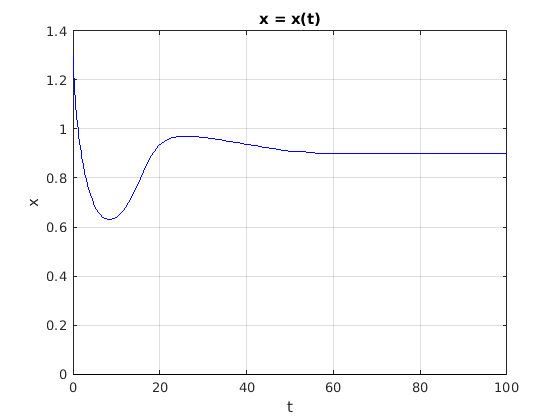
\includegraphics[width=8cm]{18_syst_equ_diff/graphe5a}
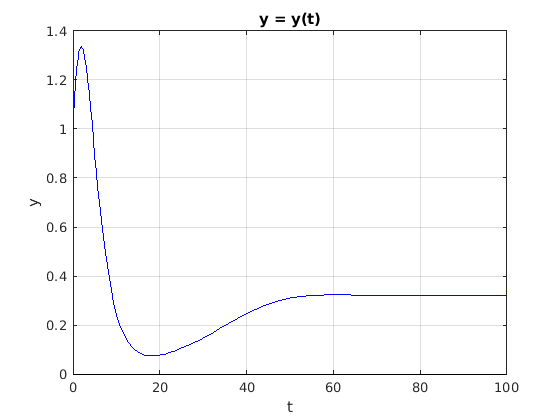
\includegraphics[width=8cm]{18_syst_equ_diff/graphe5b}
% \MATHgraph{18_syst_equ_diff/graphe5a}{8cm}
% \MATHgraph{18_syst_equ_diff/graphe5b}{8cm}

Pour observer plus d'oscillations autour du point d'équilibre
$\VEC{p}$, il faudrait intégrer pour une très longue période de
temps (puis comprimer le graphe selon l'axe des $t$ et
étirer le graphe selon l'axe des $x$ et $y$).
Qualitativement, les graphes de $x$ et $y$ devraient être semblables à
ceux qui suivent.
\PDFgraph{18_syst_equ_diff/graphe5}
}

%%% Local Variables: 
%%% mode: latex
%%% TeX-master: "notes"
%%% End: 
